\section{Results}
\label{sec:results}

% All numbers come from scripts/08_aggregate_results.py outputs: tables in
% paper/tables/*.tex, figures in paper/figures/*.pdf, and number macros in
% paper/tables/numbers.tex (e.g. \resESevenBTwoSmallFindingRecall).
% Never type a result number in this file; tests/test_paper.py checks it.

\subsection{Headline vs.\ hidden metrics}
% TODO: average accuracy holds while hidden metrics drop (H1).
\todo{headline vs hidden}

\begin{figure}[t]
  \centering
  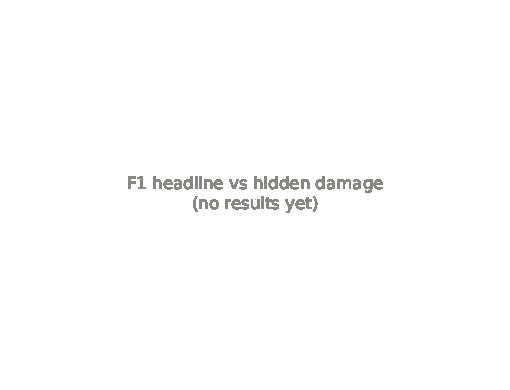
\includegraphics[width=0.48\linewidth]{figures/headline_vs_hidden.pdf}
  \caption{Headline vs.\ hidden damage: drop in accuracy against drop in
  small-finding recall relative to \expid{E2}; points above the diagonal lose
  more on small findings than on accuracy (H1).}
  \label{fig:headline}
\end{figure}

\begin{table}[t]
  \centering
  \caption{Main results: \expid{E2} reference, \expid{E3} (measured footprint) and
  \expid{E5}--\expid{E8} at \expid{B1}--\expid{B3}; mean $\pm$ SD over 3 seeds.}
  \label{tab:main}
  \resizebox{\linewidth}{!}{% GENERATED by scripts/08_aggregate_results.py from results/. Do not edit.

\begin{tabular}{llllll}
\toprule
Budget & Arm & Accuracy & Balanced acc. & Small-finding recall & Lesion-mask effect \\
\midrule
ref & E2 & -- & -- & -- & -- \\
meas. & E3:w8 & -- & -- & -- & -- \\
meas. & E3:w4 & -- & -- & -- & -- \\
meas. & E3:w8a8 & -- & -- & -- & -- \\
B1 & E5:magnitude & -- & -- & -- & -- \\
B1 & E5:activation & -- & -- & -- & -- \\
B1 & E5:taylor & -- & -- & -- & -- \\
B1 & E6 & -- & -- & -- & -- \\
B1 & E7 & -- & -- & -- & -- \\
B1 & E8 & -- & -- & -- & -- \\
B2 & E5:magnitude & -- & -- & -- & -- \\
B2 & E5:activation & -- & -- & -- & -- \\
B2 & E5:taylor & -- & -- & -- & -- \\
B2 & E6 & -- & -- & -- & -- \\
B2 & E7 & -- & -- & -- & -- \\
B2 & E8 & -- & -- & -- & -- \\
B3 & E5:magnitude & -- & -- & -- & -- \\
B3 & E5:activation & -- & -- & -- & -- \\
B3 & E5:taylor & -- & -- & -- & -- \\
B3 & E6 & -- & -- & -- & -- \\
B3 & E7 & -- & -- & -- & -- \\
B3 & E8 & -- & -- & -- & -- \\
\bottomrule
\end{tabular}
}
\end{table}

\subsection{Which compression family damages what}
% TODO: per-metric change relative to E2 (H2).
\todo{family comparison}

\begin{figure}[t]
  \centering
  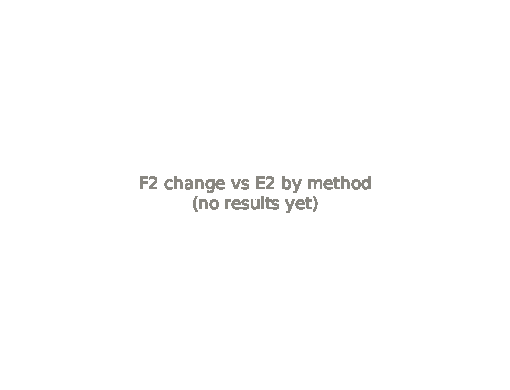
\includegraphics[width=\linewidth]{figures/family_damage.pdf}
  \caption{Change vs.\ \expid{E2} on each metric (rows) for each compressed arm
  (columns).}
  \label{fig:families}
\end{figure}

\begin{figure}[t]
  \centering
  
\includegraphics[width=0.48\linewidth]{figures/budget_curves.pdf}
  \caption{Small-finding recall against measured peak memory (fraction of
  \expid{E2}).}
  \label{fig:budgets}
\end{figure}

\subsection{Clinical vs.\ generic pruning criteria}
% TODO: primary endpoints at B2, E7 vs best of E5 and E6 (H3, Holm-corrected).
\todo{clinical vs generic}

\begin{table}[t]
  \centering
  \caption{Primary comparison at \expid{B2}: \expid{E7} minus the best of
  \expid{E5}/\expid{E6} (chosen on validation); paired bootstrap 95\% CIs and
  Holm-adjusted $p$-values.}
  \label{tab:primary}
  \resizebox{\linewidth}{!}{% GENERATED by scripts/08_aggregate_results.py from results/. Do not edit.

\begin{tabular}{lllll}
\toprule
Comparison & $\Delta$ small-finding recall [95\% CI] & $p_{\mathrm{Holm}}$ & $\Delta$ lesion-mask effect [95\% CI] & $p_{\mathrm{Holm}}$ \\
\midrule
E7 vs best of E5/E6 & -- & -- & -- & -- \\
\bottomrule
\end{tabular}
}
\end{table}

\begin{figure}[t]
  \centering
  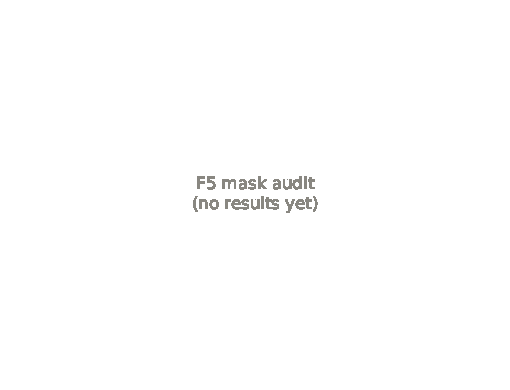
\includegraphics[width=0.48\linewidth]{figures/mask_audit.pdf}
  \caption{Mask audit: answer flip rate when the lesion is masked vs.\ an
  area-matched random region.}
  \label{fig:mask}
\end{figure}

\subsection{Ablations}
% TODO: A1-A6 at B2.
\todo{ablations}

\begin{table}[t]
  \centering
  \caption{Criterion ablations at \expid{B2}.}
  \label{tab:ablations}
  % GENERATED by scripts/08_aggregate_results.py from results/. Do not edit.

\begin{tabular}{lll}
\toprule
Arm & Small-finding recall & Lesion-mask effect \\
\midrule
E7 & -- & -- \\
A1 & -- & -- \\
A2 & -- & -- \\
A3 & -- & -- \\
A4:n32 & -- & -- \\
A4:n64 & -- & -- \\
A4:n128 & -- & -- \\
A4:n256 & -- & -- \\
A5:logprob\_drop & -- & -- \\
A5:kl & -- & -- \\
A6:layers\_only & -- & -- \\
A6:heads\_channels & -- & -- \\
\bottomrule
\end{tabular}

\end{table}

\subsection{Is accuracy a reliable guide?}
% TODO: H4.
\todo{ranking}

\begin{figure}[t]
  \centering
  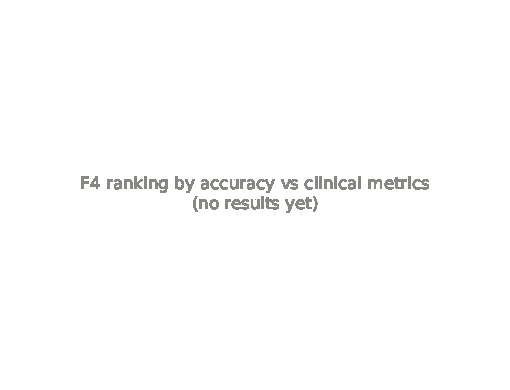
\includegraphics[width=0.48\linewidth]{figures/rank_order.pdf}
  \caption{Rank of each compressed arm by accuracy vs.\ by small-finding recall
  (H4).}
  \label{fig:rank}
\end{figure}

\subsection{Efficiency and external test}
% TODO: measured footprints; low-precision kernel check; external test.
\todo{efficiency}

\begin{table}[t]
  \centering
  \caption{Efficiency on the timing GPU (budget-matched arms at \expid{B2}).}
  \label{tab:efficiency}
  \resizebox{\linewidth}{!}{% GENERATED by scripts/08_aggregate_results.py from results/. Do not edit.

\begin{tabular}{lllllll}
\toprule
Arm & Params & File size & Peak memory & Cold latency (s) & Warm latency (s) & Kernels OK \\
\midrule
E0 & -- & -- & -- & -- & -- & -- \\
E1 & -- & -- & -- & -- & -- & -- \\
E2 & -- & -- & -- & -- & -- & -- \\
E3:w8 & -- & -- & -- & -- & -- & -- \\
E3:w4 & -- & -- & -- & -- & -- & -- \\
E3:w8a8 & -- & -- & -- & -- & -- & -- \\
E4 & -- & -- & -- & -- & -- & -- \\
E5:magnitude & -- & -- & -- & -- & -- & -- \\
E5:activation & -- & -- & -- & -- & -- & -- \\
E5:taylor & -- & -- & -- & -- & -- & -- \\
E6 & -- & -- & -- & -- & -- & -- \\
E7 & -- & -- & -- & -- & -- & -- \\
E8 & -- & -- & -- & -- & -- & -- \\
E9 & -- & -- & -- & -- & -- & -- \\
\bottomrule
\end{tabular}
}
\end{table}

\begin{table}[t]
  \centering
  \caption{External test (deduplicated against training images).}
  \label{tab:external}
  % GENERATED by scripts/08_aggregate_results.py from results/. Do not edit.

\begin{tabular}{llll}
\toprule
Arm & Accuracy & Small-finding recall & Lesion-mask effect \\
\midrule
E0 & -- & -- & -- \\
E2 & -- & -- & -- \\
E3:w8 & -- & -- & -- \\
E3:w4 & -- & -- & -- \\
E3:w8a8 & -- & -- & -- \\
E5:magnitude & -- & -- & -- \\
E5:activation & -- & -- & -- \\
E5:taylor & -- & -- & -- \\
E6 & -- & -- & -- \\
E7 & -- & -- & -- \\
\bottomrule
\end{tabular}

\end{table}
